\section{Data}
\subsection{Calibration of Polarizer Axis}
The  reference angular positions corresponding to horizontal, vertical and the $\pm 45\degree$ polarization states by determination of \textit{Brewster's} angle.  Allowing the laser to fall on a air-glass interface, the angle of incidence was gradually varied while monitoring the reflected intensity. The angle corresponding to minimum reflected intensity was identified as \textit{Brewster's}
angle, when the reflected beam becomes purely \textit{s}-polarized, allowing identification of the horizontal axis of $P_1$. Then we placed the second polarizer in front of the first, to determine the vertical angular position of the second. The data is tabulated below.
\begin{table}[h!]
\centering
\begin{tabular}{c|c|c}
 & $P_1$ & $P_2$ \\
\hline
H & $284\degree$ 
  & $222\degree - 90\degree = 132\degree$ \\
\hline
V & $284 + 90\degree = 374\degree \equiv 14\degree$ 
  & $222\degree$ \\
\hline
P & $284+ 45\degree = 329\degree$ 
  & $132\degree + 45\degree = 177\degree$ \\
\hline
M & $284- 45\degree = 239\degree$ 
  & $132\degree - 45\degree = 87\degree$ \\
\hline
\end{tabular}
\caption{Polarization angle for $P_1$ and $P_2$}
\end{table}
\subsection{Measuring Polarization of SLM}
After calibration, we put the SLM in between the polarizers. Then we varied the grey scale and for each horizontal and vertical position of $P_1$, we aligned $P_2$ into the four polarization states and noted the intensity of the transmitted light. The data is tabulated below.
\begin{table}[H]
\centering
\begin{tabular}{c c c c c c}
\toprule
Grey Value & Input ($P_1$) & $I_H$ & $I_V$ & $I_P$ & $I_M$ \\
\midrule

0   & H & 3.9 & 5.1 & 3.6 & 1.6 \\
    & P & 16.8 & 40.8 & 2.4 & 51.4 \\

\midrule

64  & H & 0.8 & 2.4 & 2.5 & 1.3 \\
    & P & 16.6 & 19.1 & 17.0 & 32.2 \\

\midrule

128 & H & 0.4 & 4.0 & 2.7 & 1.5 \\
    & P & 12.3 & 39.2 & 2.6 & 50.0 \\

\midrule

255 & H & 0.5 & 3.7 & 2.7 & 1.4 \\
    & P & 15.3 & 39.6 & 15.3 & 50.5 \\

\bottomrule
\end{tabular}
\caption{Photodetector current for different grey values and polarization states.}
\end{table}
We calculate the Stokes vector from the data above, according to the given formulas.
\begin{table}[H]
\centering
\footnotesize
\renewcommand{\arraystretch}{0.8}
\begin{tabular}{c c c}
\hline
\textbf{Grayscale} & $\mathbf{P_1}$ & \textbf{Normalized Stokes Vector} $\vb{S}$\\
\hline
0   & Horizontal (H) & $\mqty[ 1 \\ -0.133 \\ 0.222 \\ - ]$ \\
0   & +45\degree State (P)      & $\mqty[ 1 \\ -0.416 \\ -0.850 \\ - ]$ \\

\hline

64  & Horizontal (H) & $\mqty[ 1 \\ -0.5 \\ 0.375 \\ - ]$ \\
64  & +45\degree State (P)      & $\mqty[ 1 \\ -0.07 \\ -0.426 \\ - ]$ \\

\hline

128 & Horizontal (H) & $\mqty[ 1 \\ -0.818 \\ 0.273 \\ - ]$ \\
128 & +45\degree State (P)      & $\mqty[ 1 \\ -0.522 \\ -0.920 \\ - ]$ \\

\hline

255 & Horizontal (H) & $\mqty[ 1 \\ -0.761 \\ 0.309 \\ - ]$ \\
255 & +45\degree State (P)      & $\mqty[ 1 \\ -0.443 \\ -0.641 \\ - ]$ \\

\hline
\end{tabular}
\caption{Normalized Stokes Vectors for Different Grayscale values}
\end{table}
\noindent
We then calculated $X$ and $Y$, from which we obtained $\delta$ and $\psi$, using the formulas mentioned before and then the extracted linear retardance and optical rotation were plotted as functions of greyscale values. 
\begin{figure}[H]
  \centering 
  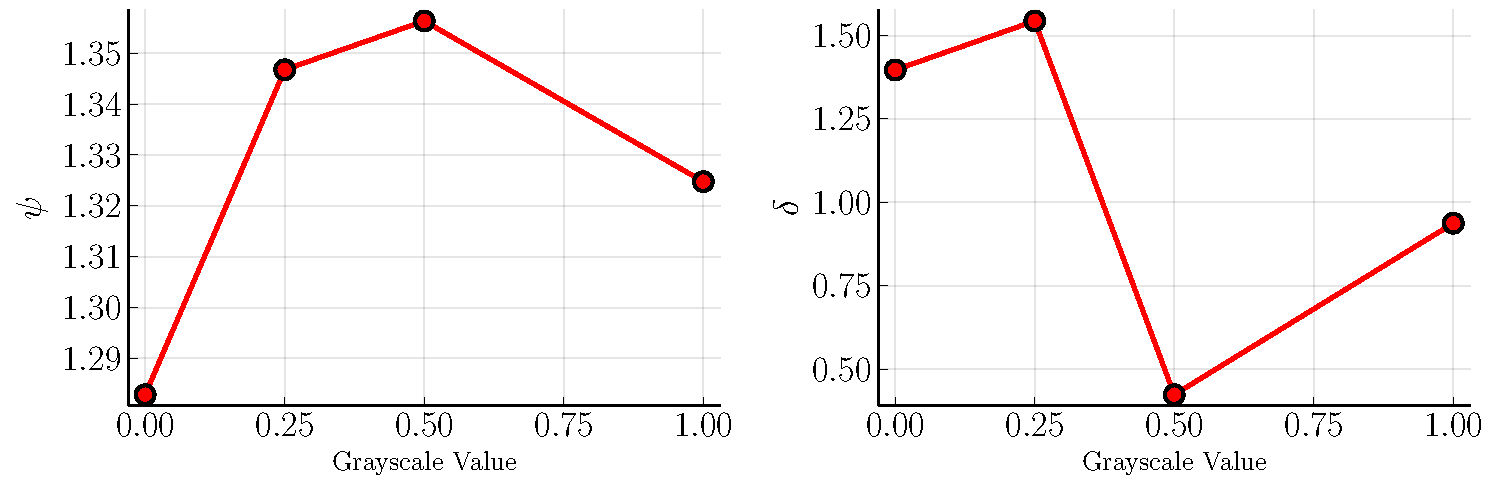
\includegraphics[width=0.9\textwidth]{SLM1.pdf}
\end{figure}

